\section{Integrated Sensors}\label{Sensors}
\subsection{Verwendete Sensoren}
Im Projekt werden zwei Sensoren benötigt. Zum einen ein Temperatursensor und zum anderen ein Strommesser. Der Temperatursensor wurde an dem Raspberry-Pi angeschlossen, um die Temperatur in einem Raum messen zu können.
Der Stromsensor wurde an den Mikrocontroller angeschlossen, um feststellen zu können wann der Motor am Ende seiner Umdrehungsmöglichkeit angekommen ist.

\subsection{Temperatursensor}
Um die Temperatur messen zu können, wird ein Temperatursensor benötigt. Wenn ein Temperatursensor an einen Mikrokontroller angeschlossen werden soll, wird ein analoger Temperatursensor benötigt, der die Temperatur beispielsweise in eine Spannung oder einen Strom umwandelt. Des Weiteren ist einen AD-Wandler nötig, der das Signal digitalisiert. Dieser kann auf dem Sensor oder dem Mikrocontroller integriert sein.

Temperatursensoren gibt es in verschiedenen Varianten. Vom temperaturabhängigen Widerstand bis zum fertig abgeglichenen All-in-one-Bauteil mit digitalem Ausgang.

Im Projekt wurden zwei verschiedene Sensoren getestet.

\subsubsection{Sunfounder - Analog Temperatur Sensor Module}
\paragraph{Beschreibung}\mbox{}\\
Der Temperatursensor von Sunfounder weist eine hohe Genauigkeit der Messung durch eine große Reichweite auf, außerdem besitzt er eine gute Stabilität sowie eine starke Überladungskapazität. Der Sensor kann analoge und digitale Signale gleichzeitig ausgeben (siehe \Abbildung{sensors1}).

\begin{figure}[H]
\centering
\includegraphicsKeepAspectRatio{sensors/SunFounder.png}{0.4}
\caption{Sunfounder - Analog Temperatur Sensor Module}
\label{fig:sensors1}
\end{figure}

\paragraph{Technische Daten}\mbox{}\\
\begin{itemize}
\item NTC Thermistor
\item LM393
\item Potentiometer
\item PCB 2.3 x 2.3 cm
\item Betriebsspannung: 3.3V-5V
\end{itemize}

\subsubsection{Seeedstudio - Temperatur Sensor Daten}
\paragraph{Beschreibung}\mbox{}\\
Der Temperatursensor von Seeedstudio besitzt einen Delta-Sigma-Analog-Digital Converter. Durch den I2C Port kann der Sensor mit dem Raspberry Pi kommunizieren, dabei hat jedes angeschlossene Gerät eine eigene Adresse (siehe \Abbildung{sensors2}).

\begin{figure}[H]
\centering
\includegraphicsKeepAspectRatio{sensors/SeedSensor.png}{0.4}
\caption{Seeedstudio - Temperatur Sensor Daten}
\label{fig:sensors2}
\end{figure}

\paragraph{Technische Daten}\mbox{}\\
\begin{itemize}
\item Temperaturbereich von -25°C~100°C
\item PCB 1.3 x 1.0 cm
\item Betriebsspannung: 3.3V-5V
\item unterstützt Raspberry Pi und Arduino
\item kompatibel mit Raspberry Pi A+,B,B+/2
\item I2C Port
\item LM75 IC
\end{itemize}

\subsubsection{Problemstellung}
Wurde der Temperatursensor direkt auf dem Pi geschlossen, gab dieser zunächst falsche Temperaturwerte zurück (siehe \Abbildung{sensors3}).

\begin{figure}[H]
\centering
%\includegraphicsKeepAspectRatio{sensors/3.jpg}{0.6}
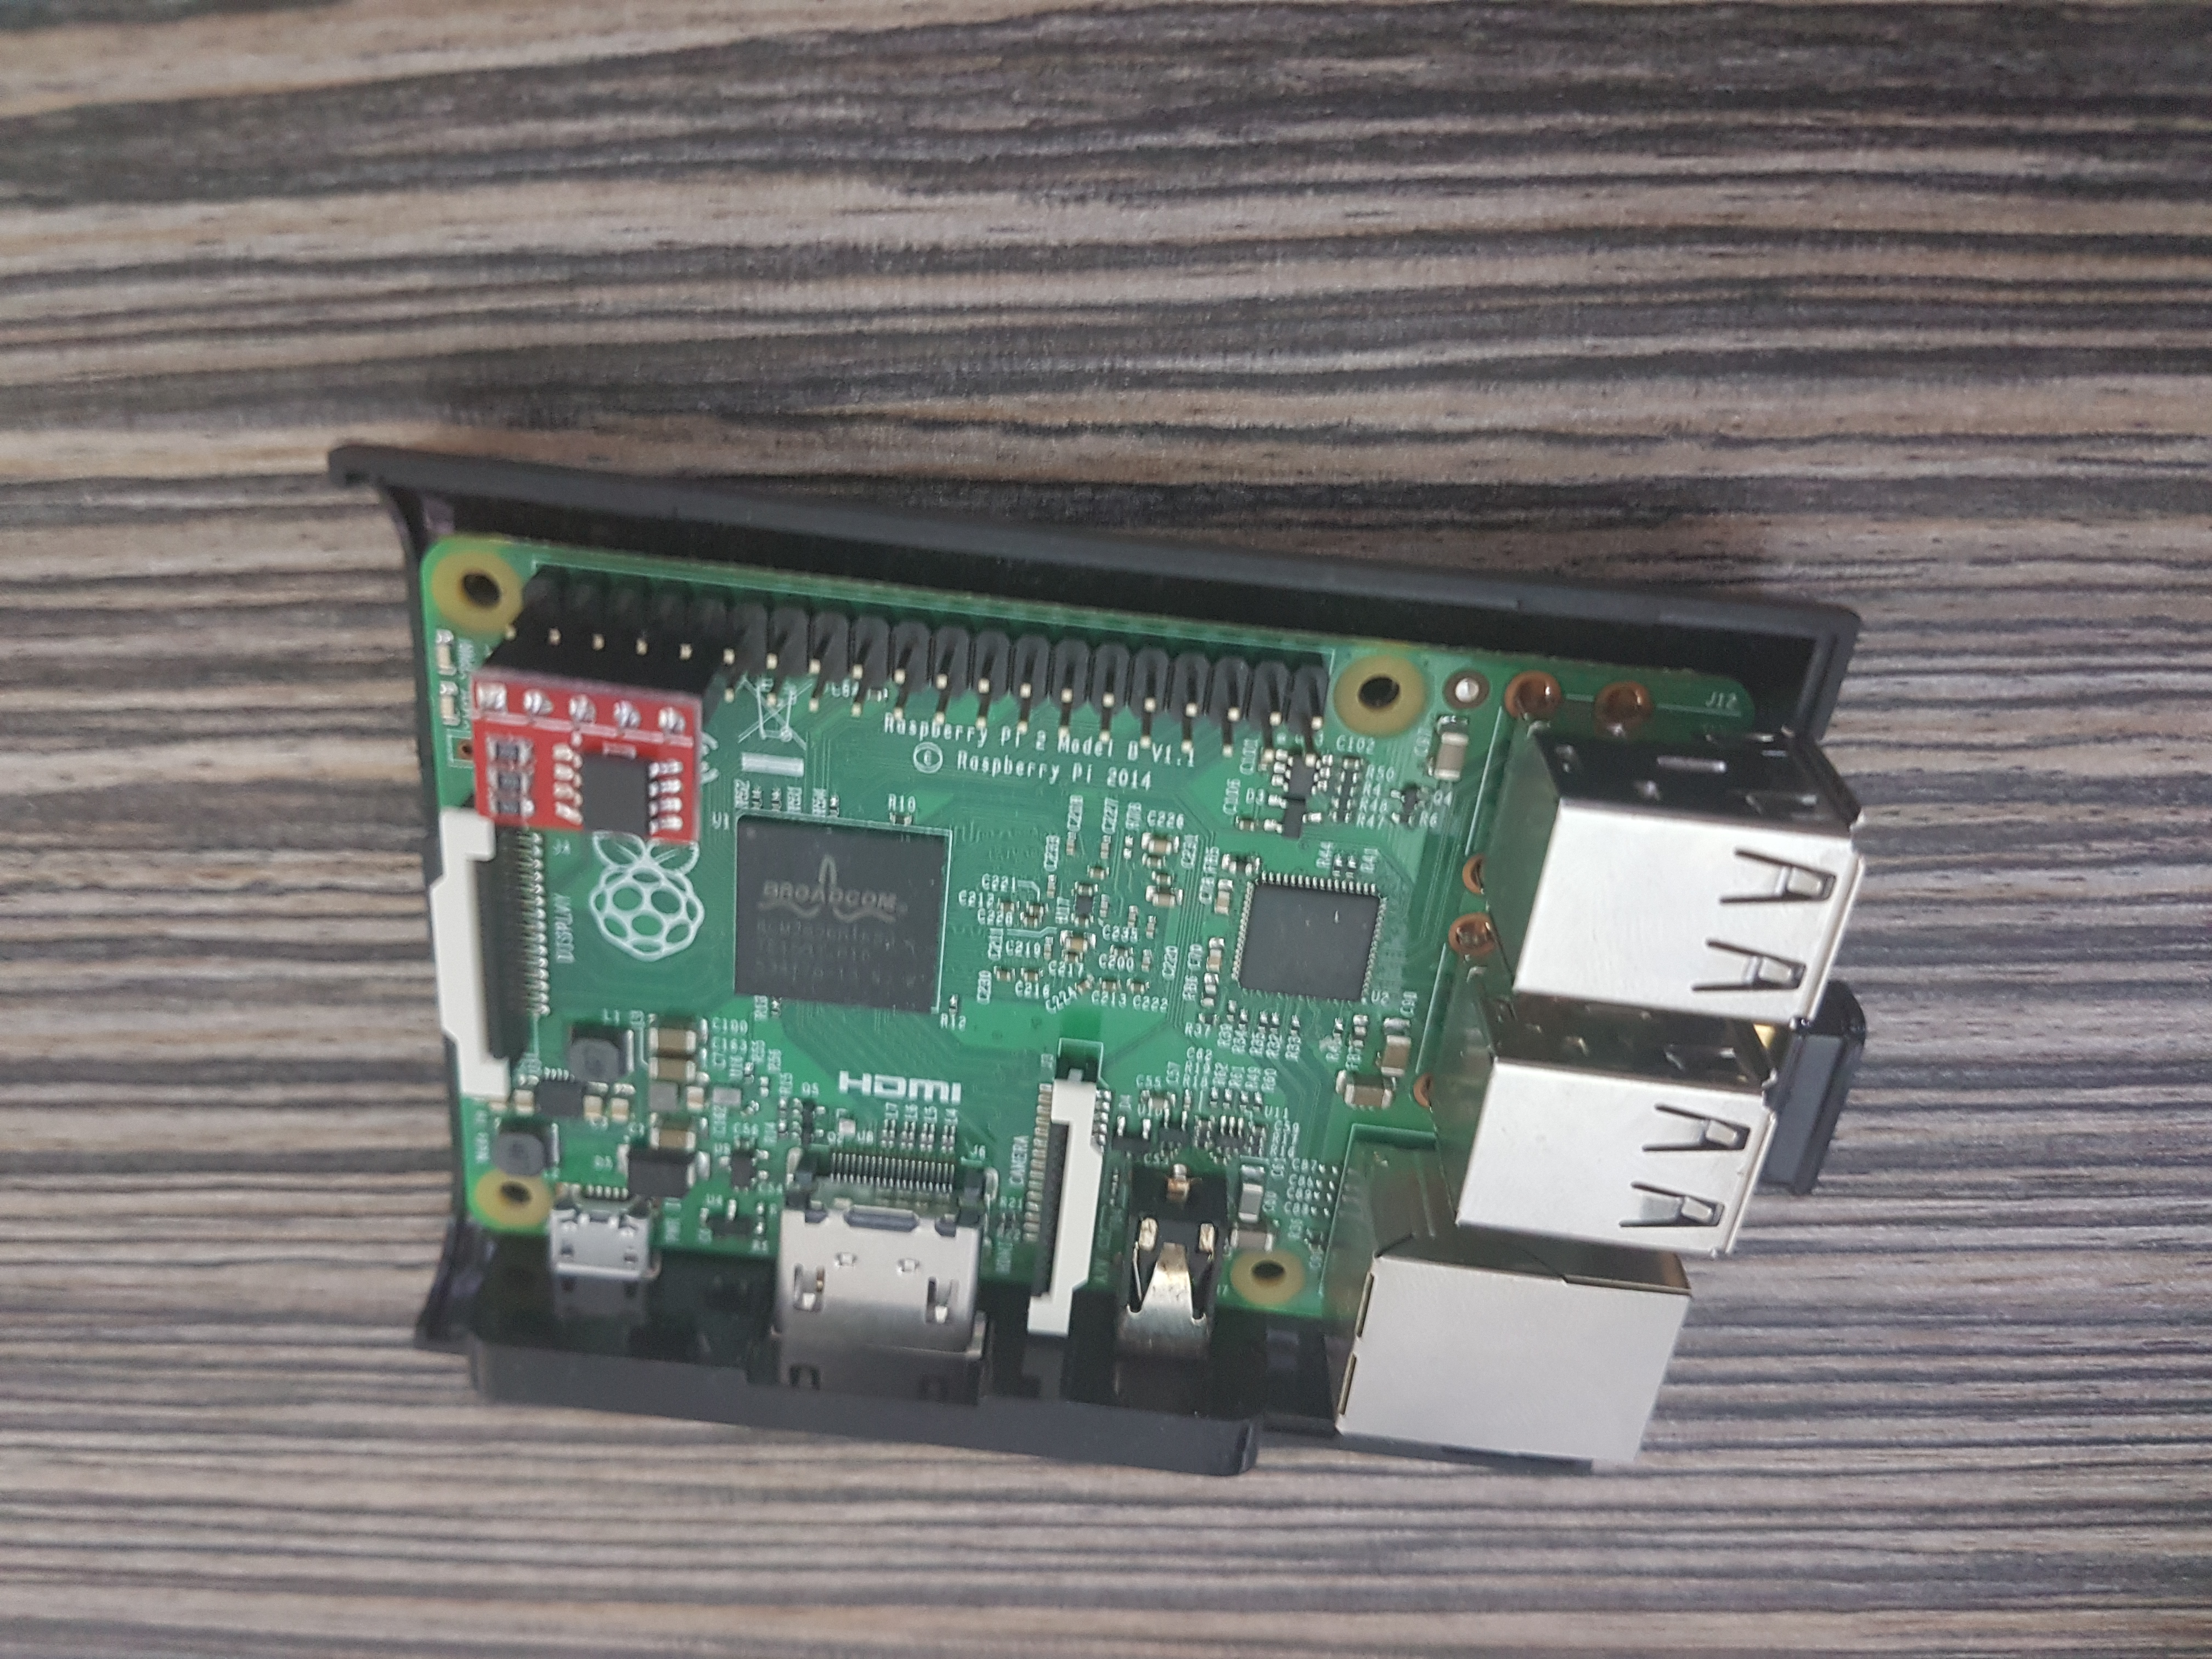
\includegraphics[angle=180,scale=0.06]{sensors/3.jpg}
\caption{Temperatursensor am Pi}
\label{fig:sensors3}
\end{figure}

Diese entstanden jedoch nicht durch eine falsche Pin-Belegung oder durch ungenaues Messen des Sensors, sondern daran, dass sich die Temperatur durch die Hardware des Pi im Laufe des Betriebs erhöhte und eine hohe Wärme abgab. Diese erwärmte Luft im direkten Umfeld des Pi’s sorgte dafür, dass zu dieser Zeit der Wärmewert der Luft so hoch war, dass dieser die Messwerte verfälschte.

Abhilfe wurde dadurch geschaffen, dass der Sensor in einem Bereich in dem die erwärmte Luft durch die Pi Hardware nicht mehr relevant war ausgelagert wurde (\Abbildung{sensors4}).

\begin{figure}[H]
\centering
\includegraphicsKeepAspectRatio{sensors/4.jpg}{0.4}
\caption{Temperatursensor am Pi mit Kabel}
\label{fig:sensors4}
\end{figure}

\subsection{Stromsensor}
\paragraph{Beschreibung}\mbox{}\\
Der ACS712 ist ein Hall-Effekt Sensor. Das heißt; wird der Sensor von einem Strom durchflossen erzeugt es in seinem Magnetfeld eine Ausgangsspannung die proportional zum Produkt aus magnetischer Feldstärke und Strom ist (das nennt man den Hall-Effekt). Der ACS712 braucht eine eigene Stromverbindung, damit er den Betrieb aufnehmen kann. Dazu besitzt er einen VCC-Pin und einen GND-Pin, welche jeweils außen sind. Um den eingehenden Strom über die oberen Kontakte auslesen zu können, ist der Out-Pin in der Mitte zuständig. Der Wert der über den Out-Pin übermittelt wird ist analog, d.h. er gibt die Werte zwischen 0-1023 aus, da die Ausgangsspannung wie oben beschrieben proportional zum Produkt aus magnetischer Feldstärke und Strom ist, liegt der Wert im Bereich zwischen 518-522, da der Sensor temperaturabhängig ist und einen Offset haben kann.


\paragraph{Technische Daten}\mbox{}\\
\begin{itemize}
\item Geräuscharmer analoger Signalweg
\item Bandbreite wird über den FILTER-Pin eingestellt
\item 5 $\mu$s Reaktion zum Eingangsstrom • 80 kHz Bandbreite
\item Abweichungsanfälligkeit 1.5\% at TA = 25°C
\item Geringer Platzbedarf, low-profile SOIC8 Gehäuse
\item 1.2 m$\Omega$ interner Leistungswiderstand
\item 2.1 kVRMS minimale Isolationsspannung an den Pins 1-4 auf die Pins 5-8
\item 5.0 V Einzelbetrieb
\item 66 bis 185 mV/A Ausgangsempfindlichkeit
\item Ausgangsspannung proportional zum Fluss AC oder DC
\item Stabile Ausgangsoffsetspannung
\item Magnet Hysterese knapp bei Null
\end{itemize}


\subsection{Im Projekt Hausautomatisierung}
Verwendung: Das 5a Range Current Sensor Module Acs712 Module wird in unserem Projekt dazu verwendet, um die Stromspannung die der Motor bekommt / abgibt zu messen. Wenn der Motor auf einen Widerstand trifft, steigt die Stromstärke. Diese wird im Atmega-88 ausgelesen und ausgewertet, übersteigt die Stromstärke einen festgelegten Schwellenwert, wird die Stromzufuhr für den Motor abgestellt. Damit die Stromstärke ausgehend vom Motor ausgelesen werden kann, ist der Sensor mit dem Motor in Reihe geschaltet.